\section{Experimental Design}

This section describes the platform and simulator (5.1), the scenarios (5.2), the tuning of the controllers and the filter gain (5.3), the evaluation protocol (5.4), the metrics (5.5), and the hypotheses and analysis (5.6).

\subsection{Platform and simulation}

The robot is a four-wheel mecanum base derived from the KUKA youBot. It is holonomic: it can translate in any direction and rotate independently. Let $(x, y, \psi)$ be its pose in the world frame, with heading $\psi$, and let $u = (v_x, v_y, \omega)$ be the body twist, with $v_x$ forward, $v_y$ to the left and $\omega$ the yaw rate. The controller issues $u$ at a control period of $\Delta t = 0.05$ s. The pose evolves as

\begin{equation*}
\dot x = v_x \cos\psi - v_y \sin\psi, \qquad
\dot y = v_x \sin\psi + v_y \cos\psi, \qquad
\dot\psi = \omega .
\tag{9}
\end{equation*}

\emph{Wheel kinematics.} Let $r_w = 0.05$ m be the wheel radius, $l = 0.228$ m the half wheelbase and $w = 0.1585$ m the half track, and define the lever arm $L = l + w = 0.3865$ m. With the wheels ordered front-left, front-right, rear-left and rear-right, the wheel angular speeds $\boldsymbol{\varpi} = (\varpi_{\mathrm{fl}}, \varpi_{\mathrm{fr}}, \varpi_{\mathrm{rl}}, \varpi_{\mathrm{rr}})^{\top}$ that realise a twist are given by the mecanum mixing

\begin{equation*}
\boldsymbol{\varpi} = \frac{1}{r_w}\, \mathbf{S}
\begin{pmatrix} v_x \\ v_y \\ L\,\omega \end{pmatrix}, \qquad
\mathbf{S} =
\begin{pmatrix}
1 & -1 & -1 \\
1 & \phantom{-}1 & \phantom{-}1 \\
1 & \phantom{-}1 & -1 \\
1 & -1 & \phantom{-}1
\end{pmatrix}.
\tag{10}
\end{equation*}

A per-wheel sign, fixed by the orientation of the joints in the scene, multiplies each entry and is omitted here. The columns of $\mathbf{S}$ are orthogonal and each has squared norm 4, so $\mathbf{S}^{\top}\mathbf{S} = 4\,\mathbf{I}$, and the twist is recovered from measured wheel speeds by the left inverse

\begin{equation*}
\begin{pmatrix} v_x \\ v_y \\ L\,\omega \end{pmatrix} = \frac{r_w}{4}\, \mathbf{S}^{\top} \boldsymbol{\varpi}.
\tag{11}
\end{equation*}

The rim speed of wheel $i$ is $r_w|\varpi_i|$. Each row of $\mathbf{S}$ combines $v_x$, $v_y$ and $L\omega$ with signs, and the four rows realise every sign pattern of $(v_y, L\omega)$ relative to $v_x$. The fastest wheel therefore has rim speed $\max_i r_w|\varpi_i| = |v_x| + |v_y| + L|\omega|$, and the wheel-speed limit is the polytope

\begin{equation*}
|v_x| + |v_y| + L\,|\omega| \ \le\ f\, v_{\mathrm{rim}},
\tag{12}
\end{equation*}

where $v_{\mathrm{rim}} = 0.617$ m/s is the measured rim-speed ceiling and $f = 0.95$ is the share available to the filter's output. A command that violates (12) is multiplied by a single factor, so that it keeps its direction in all three components and only slows.

\emph{Command limits.} The twist is also confined to an axis box, $|v_x|, |v_y| \le 0.5$ m/s and $|\omega| \le 1.5$ rad/s. The translational pair is scaled along its own direction by the largest factor $s \le 1$ that satisfies $|s v_x| \le 0.5$ and $|s v_y| \le 0.5$, and the yaw rate is clipped separately:

\begin{equation*}
(v_x, v_y) \leftarrow s\,(v_x, v_y), \qquad \omega \leftarrow \mathrm{clip}(\omega, -1.5, 1.5).
\tag{13}
\end{equation*}

An acceleration limiter bounds every change of the applied command with respect to the previously applied one, $u_{k-1}$. The limit on the translational change is isotropic and depends on whether the planar speed decreases:

\begin{equation*}
\big\|(v_x, v_y)_k - (v_x, v_y)_{k-1}\big\| \le
\begin{cases}
a_{\mathrm{dec}}\,\Delta t & \text{if the planar speed decreases},\\
a_{\max}\,\Delta t & \text{otherwise},
\end{cases}
\qquad |\omega_k - \omega_{k-1}| \le \alpha_{\max}\,\Delta t,
\tag{14}
\end{equation*}

with $a_{\max} = 0.5$ m/s$^2$, $a_{\mathrm{dec}} = 1.0$ m/s$^2$ and $\alpha_{\max} = 1.4$ rad/s$^2$. These bounds are not properties of the youBot. They are specified together with the protective fields, so that no speed band can be skipped within one reach time and the robot cannot brake harder than the fields assume. The safety layers use the estimated body velocity $\hat v$, obtained from differenced poses with a low-pass filter of time constant 0.10 s.

\emph{Footprint.} The footprint is a measured table $e(\psi)$, the distance from the body origin to the envelope of every part that can strike an obstacle along each bearing $\psi$, with inscribed and circumscribed radii of 0.209 m and 0.3374 m. Measured quantities are configured at the upper bound of their measurement bracket, because understating a safety footprint is the unsafe direction.

Two scanners of the SICK S300 type sit on diagonally opposite corners and cover 270$^\circ$ each, so that together they see everything outside the outline. The scan plane lies 0.2206 m above the floor. The returns are binned inside the simulator into a policy stream of 36 sectors of 10$^\circ$ and a filter stream of 120 sectors of 3$^\circ$. Each sector carries its minimum range in [0.05, 5.0] m, its bearing and a validity flag. A sector is valid only if its whole extent, from the footprint edge to 1.0 m beyond it, is seen by some sensor. An invalid sector breaches every certified field.

The experiments run in CoppeliaSim 4.10 with the ODE engine at a dynamics step of 0.005 s \cite{rohmer2013vrep}. The engine is a stated condition: in a declared sweep, the same model's heading drift over a 5 m lateral profile was 20.55$^\circ$ under Bullet, 0.47$^\circ$ under ODE and 3.12$^\circ$ under Newton. Scanners are processed inside the simulator and published as one packet per control step. Determinism is claimed within one scene load only. Every run records its commit, host, scene hash and resolved configuration.

\subsection{Scenarios}

\emph{Layouts.} Each scenario is a procedurally generated warehouse hall with perimeter walls and two to four rows of shelving taller than the scan plane. Aisles are stratified by per-side clearance, the gap on each side of a centred robot: narrow [0.1987, 0.2687) m, medium [0.2687, 0.40) m and wide [0.40, 0.80] m. The narrow floor follows a declared rule: it is the smallest clearance at which the at-rest and moving fields of a robot displaced by the committed tracking bound remain clear of the walls, plus a 0.03 m buffer. Start and goal are drawn so that at least 1.5 m of the route lies in an aisle. Every route must be traversable by an oracle tracker that keeps the lowest band's field clear from start to goal. When this check fails, the goal is redrawn, never the layout.

\emph{Obstacles absent from the map.} The central condition of the study is a world that differs from the map. Unmapped obstacles, square boxes of 0.25 to 0.60 m taller than the scan plane, are placed relative to the planned route: the first at an offset uniform on [0, 0.3] m from the route to its nearest surface, any second on [0, 0.6] m. An obstacle is kept only if the robot could pass it within 1.0 m of the route, judged jointly with the obstacles already placed, since the stack does not replan. The planner never sees these obstacles. The scanners and the safety layers do.

\emph{Route and map.} Each layout is rasterised into a 0.05 m grid from which unmapped obstacles are excluded. Cells within the inscribed half-width plus 0.10 m (0.3086 m) of an obstacle are lethal, and a soft cost falls linearly from there to the circumscribed radius plus 0.03 m. An 8-connected A$^{*}$ search finds the cheapest path (Figure~\ref{fig:layouts}). A controller receives a lookahead point 0.8 m ahead on this route and the goal, both in the body frame.

\begin{figure}[t]
\centering
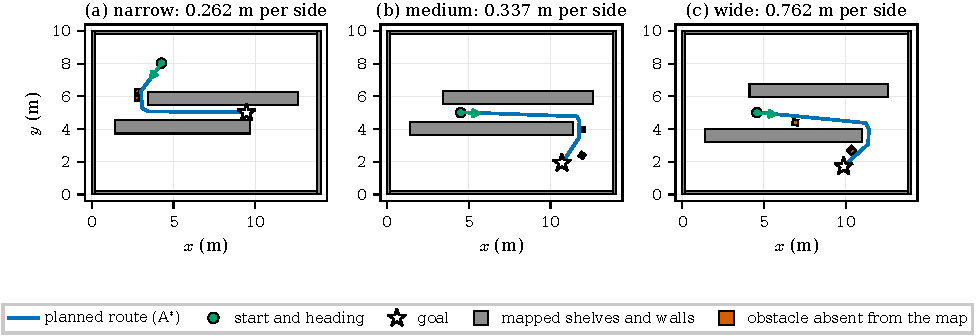
\includegraphics[width=\linewidth]{fig4_layout.pdf}
\caption{Example scenarios, one for each aisle stratum, from the tuning set: (a) narrow, (b) medium and (c) wide, with per-side clearances of 0.262, 0.337 and 0.762~m. Grey rectangles are mapped shelves and walls. Orange squares are obstacles that are absent from the planner's map but present in the world and visible to the scanners. The blue line is the A$^*$ route planned on the map, the green dot with an arrow is the start position and heading, and the star is the goal.}
\label{fig:layouts}
\end{figure}

\emph{Scenario sets.} Layouts are identified by seed, geometry hash and generator hash, regenerated and verified at load, and drawn from disjoint seed ranges (Table~\ref{tab:sets}).

\begin{table}[t]
\caption{Scenario sets. Layouts are drawn from disjoint seed ranges.}
\label{tab:sets}
\centering
\small
\begin{tabular}{lp{5.6cm}p{4.4cm}}
\toprule
Set & Size & Purpose \\
\midrule
Tuning & 60 scenarios (20 per stratum), 633 m planned; 17 contain one or two unmapped obstacles & controller tuning and the gain sensitivity \\
Validation & 180 scenarios, 30 in each of 6 cells (mapped-only and unmapped $\times$ narrow, medium, wide), never trained on & development reporting only; no model or hyperparameter is selected on it \\
Test (sealed) & 300 scenarios: 50 in each of 3 strata $\times$ 2 conditions (mapped-only; one unmapped obstacle on every route); 1,606 m and 1,624 m planned & the confirmatory evaluation, run once \\
\bottomrule
\end{tabular}
\end{table}

The test set was built and locked before any controller was evaluated on it. B1, B2 and B3 alone, and B2 with the filter, were each evaluated once on both of its halves. Test layouts are never used for tuning, debugging, reward design or plots during development.

\subsection{Controller tuning and the filter gain}

Each classical controller is tuned alone, on the tuning scenarios only, by a random search over declared parameter ranges. Every controller receives the same number of candidates. The first candidate of B3 takes the Nav2 DWB defaults. The filtered controller keeps the tuned parameters of its host unchanged, so that a comparison of a controller with and without the filter differs only in the filter.

The filter gain $\alpha$ is frozen at 1.0 s$^{-1}$ for every filtered controller. To show how the stops depend on it, we report a sensitivity analysis on the tuning scenarios for the grid $\alpha \in \{1, 2, 5, 10, 20\}$ s$^{-1}$ with B2 + PFB (Section 6.3). The value 1.0 is the lowest of the grid, and it is not selected as an optimum. The runs use seed 0 on the earlier training host, and are not repeated on the final host.

\subsection{Evaluation protocol}

Each classical controller runs once per scenario, alone and with the filter, within one scene load, so that the two versions see the same layout and the same scan noise. The certified layer is beneath every controller, and the filtered version has the filter above it. A paired comparison uses the same scenarios in the same order, within one scene load. The runs reported here use one run per controller and condition, so they carry no estimate of run-to-run variation beyond the scenario resampling described in Section 5.6, and we state this wherever a result depends on it.

\subsection{Metrics}

Protective stops per 100 m of planned route normalises the number of modeled protective stops by the spatial extent of the task, and it is an operational measure of how often the field intervenes. We use the planned length because it is the same for every controller, so that a controller cannot lower its rate by wandering. The rate is reported beside the success rate, the timeout rate and the mission time, so that a reduction in stops is not read apart from the overall navigation performance. A stop is counted as defined in Section 3.2: a persisting breach and its latch count once, and a breach after a restart counts again. All protective stops are events of the emulated layer. No physical certified scanner is used, and the results make no claim about the behaviour of a certified physical system.

The primary endpoint is protective stops per 100 m of planned route, Eq. (5), pooled over episodes. Stops decided on a corrupted scan packet that the plausibility check replaced by the fail-safe (scan-fault stops) are excluded from the count and reported beside it. The secondary measures are the success rate, the timeout rate and the rate of unrecoverable stops, in which an episode reaches its horizon while a stop is latched and the robot cannot legally move again, so that it is distinguished from a timeout in which the robot was free to move. Contact episodes are decided by the simulator's collision check alone. Stops are also reported per 100 m driven and per 100 m on completed routes only, and the mission time, the share of time latched and the moving speed (the mean speed while not latched) are reported. For the filtered controllers, we report the share of steps on which the filter changed the command and the share on which no regime was feasible. We also report the intervention magnitude, the norm $\|(u_{\mathrm{nom}} - u_{\mathrm{PFB}}) \oslash c\|$ of the correction normalised by the axis ceilings $c$, as its mean and maximum over steps, and the 95th percentile of the filter's computation time per step.

Success and timeouts are reported beside every stop rate, because a controller can lower its stop count by moving little or by stalling.

\subsection{Hypotheses and analysis}

\emph{HF-c} (confirmatory, a family of its own): B2 + PFB triggers fewer protective stops per 100 m of planned route than B2 alone, on the test condition with an unmapped obstacle on every route, strata pooled, each arm run once per scenario. The claim is stop removal only. Success, mission time, latched share and moving speed are reported beside it, descriptively and without inference. All other comparisons are exploratory and are labelled as such: the filter beneath B1 and B3 against each alone, the constant-margin comparator of Section 4.4 \tbd{not yet run}, and the sensitivity to $\alpha$. The classical results in Section 6.1 come from the validation sets and are exploratory. HF-c was evaluated once on the sealed test set, and Section 6.2 reports it.

Table~\ref{tab:comparisons} states what each comparison establishes.

\begin{table}[t]
\caption{What each comparison establishes. HF-c is confirmatory; the others are exploratory.}
\label{tab:comparisons}
\centering
\small
\begin{tabular}{p{4.2cm}p{8.0cm}}
\toprule
Comparison & What it establishes \\
\midrule
B2 vs.\ B2 + PFB & effect of the filter on a classical controller (HF-c) \\
B1, B3 vs.\ each with PFB & whether the effect holds across classical controllers \\
PFB vs.\ constant-margin filter & whether the speed- and direction-dependent field matters \tbd{not yet run} \\
\bottomrule
\end{tabular}
\end{table}

\emph{Estimand and interval.} The estimand is the rate ratio of protective stops, total stops over total planned length per arm, with 0.5 added to each arm's stop count:

\begin{equation*}
\widehat{\mathrm{RR}}_{AB} = \frac{(S_A + 0.5)/\Lambda_A}{(S_B + 0.5)/\Lambda_B},
\tag{15}
\end{equation*}

where $S$ is the pooled stop count and $\Lambda$ the pooled planned length. The interval is a bootstrap of $\log \widehat{\mathrm{RR}}$ in which scenarios are resampled jointly across arms. A classical controller runs once, so its interval has the scenario part alone, with a $t$ quantile on $n - 1$ degrees of freedom. A comparison rejects when the two-sided interval lies wholly below zero on the log scale, and HF-c is tested at the level 0.05. Before the interval was used, its rejection rate at equal true rates was checked on synthetic data, with 150 route pairs, the pilot route lengths and 10,000 replications, over stop rates of 0.5, 1, 2, 5 and 52.8 per 100~m and two levels of difficulty. The gate required the one-sided rejection rate on each side to stay within 0.025 plus three Monte Carlo standard errors, 0.0297. All ten cells passed, the highest rejection rate being 0.0274, and the check was made before the test set was read. The cells at 0.25 stops per 100~m, which lie below the rates of the arms here, were reported and not gated, and a few of them exceeded the bound slightly.

\emph{Power.} At the stop rates seen on the development set, a rate ratio of about 0.009, the power of HF-c at 150 scenarios is close to one, so power did not constrain the test size. We do not weaken the comparison: the rate-ratio interval is reported in any case, and the outcome is labelled inconclusive if the interval includes one. The locked test set will not be enlarged.

\emph{Disclosure.} The test size and HF-c as a confirmatory comparison were fixed before the test set was built or read, but after development-set stop rates had been seen. The comparisons of the filter beneath B1 and B3 were proposed after the test set had been read for other controllers, and nothing about them is confirmatory.
